
\resetcounters

\bibliographystyle{asp2010}

\markboth{Becker, Winkelman, and Rots}{Better Living Through Metadata}

\title{Better Living Through Metadata: Examining Archive Usage}
\author{Glenn~Becker,$^1$ Sherry~Winkelman,$^1$ and Arnold~Rots$^1$}
\affil{$^1$Smithsonian Astrophysical Observatory, 60 Garden Street, Cambridge, MA 02138}

\aindex{Becker, G.}
\aindex{Winkelman, S.}
\aindex{Rots, A.}

\begin{abstract}
The primary purpose of an observatory's archive is to provide access to the data through 
various interfaces. User interactions with the archive are recorded in server logs, which 
can be used to answer basic questions like: Who has downloaded dataset X? When did she 
do this? Which tools did she use? The answers to questions like these fill in patterns 
of data access (e.g., how many times dataset X has been downloaded in the past three years). 
Analysis of server logs provides metrics of archive usage and provides feedback on interface 
use which can be used to guide future interface development.

The Chandra X-ray Observatory is fortunate in that a database to track data access and 
downloads has been continuously recording such transactions for years; however, it is 
overdue for an update. We will detail changes we hope to effect and the differences 
the changes may make to our usage metadata picture. We plan to gather more information 
about the geographic location of users without compromising privacy; create improved 
archive statistics; and track and assess the impact of web "crawlers" and other scripted 
access methods on the archive. With the improvements to our download tracking we hope to 
gain a better understanding of the dissemination of Chandra's data; how effectively it 
is being done; and perhaps discover ideas for new services.
\end{abstract}

\section{Introduction}

Over the thirteen years of the Chandra mission the data in the downloads tracking database 
have yielded useful statistics about large-scale data usage and trends. Recently, we have
decided to drill down further to gather more detailed information in order to be able to 
more accurately chart and tabulate how the data is accessed, by whom, and at what rate.

To accomplish this we are making changes to the downloads database tables to 
incorporate both historical data harvested from server logs and new data obtained through online
services. The changes have so far been incremental rather than sweeping, yet they already 
allow for the creation of plots that reveal regional statistics and trends through time.

We are still at the early stages of gathering accurate geographical and other 
descriptive information about our users: where they are from, how they connect, and what they 
download. The downloads data used in this study are a snapshot from October 11, 2012, which 
is when data from the original downloads database was inserted into the revised tables.

\section{Host - IP Mining}

\begin{figure}[H]
\begin{center}
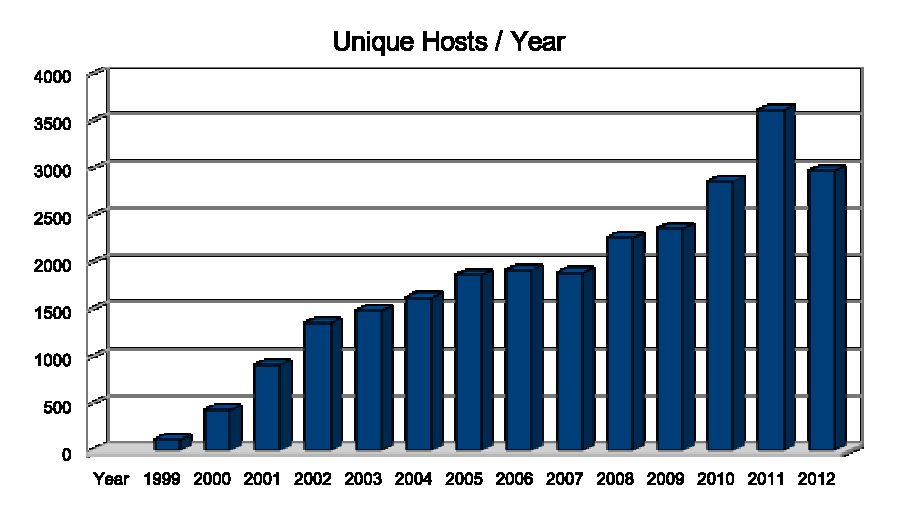
\includegraphics[width=100mm]{part6/Becker_P41/hosts_year.eps}
\end{center}
\caption{An illustration of how the number of unique hostnames / year (including all host
types) downloading data has gone steadily up through the course of the mission. There is a
downturn for 2012 since that year is not yet complete.}
\label{fig:HostsByYear}
\end{figure}

As Figure~\ref{fig:HostsByYear} displays graphically, the number of unique hosts accessing the archive
has gone up yearly. Unfortunately, the system sometimes records only partial hostnames: we have, so far, resolved 
26,000 reliable hostnames out of a total of just over 45,000 unique records. Repair of partial hostnames was 
accomplished by searching a large collection of historical logfiles. The remaining 19,000 are 
in progress; some may never be resolved. We have collected geographical information about the 
hostnames we have resolved. To accomplish this, we have:

\begin{itemize}

\item collected corresponding IP addresses where they were available in logfiles;

\item utilized UNIX 'host' and/or 'dig' commands programmatically (using Perl) to resolve alphanumeric
hostnames into numeric IP addresses;

\item determined that use of command line 'whois' to resolve IP addresses was:

\begin{enumerate}

\item problematic to parse efficiently;

\item throttled by regional Internet registries (RIR) \footnote{There are 
five regional Internet registries: ARIN (North America), RIPE (Europe), 
AFRINIC (Africa), LACNIC (South / Latin America) and APNIC (Asia / 
Oceania).};

\end{enumerate}

\item determined that RIR web presences and/or interfaces were not uniform in functionality or
completeness;

\item evaluated online commercial IP geo\-location services, offering a database 
to download or a scriptable web service (similar free services exist, but these 
typically offer dated snapshots of the full database), and chose 
MaxMind \footnote{\url{http://www.maxmind.com}}.

\end{itemize}

\section{Getting Geographic}

Once the extended user information from MaxMind had been added to the database, we
were ready to do some initial analysis and querying. An obvious first choice was download
size by country. Bots and mirror sites, identified with the aid of the MaxMind data, were
excluded from this tally.

Downloads were recorded for a total of 109 countries. Figure~\ref{fig:DownloadsByCountry} graphically displays counts
for the top 12, plus three aggregates. In terms of raw numbers, the country chart holds 
few surprises; however, it at least hints at the kind of analysis that can be done once 
the geographical information is accessible in the database.

We could, for example, present charts showing breakouts by U.S. states or general regions,
or continents, or use different criteria for the breakout (raw number of downloads, for example,
rather than total data downloaded). It would also be straightforward to track the changes
in activity through time.

There are other possibilities as well. Some of the interesting additional fields that the MaxMind 
'Omni' service returns are: metro code, time zone, ISP, organization, netspeed (Internet
connection type), user type ('searchEngineSpider' is one very useful classification here), and
more. This richness of information allows one to imagine a wealth of useful queries.

\begin{figure}[H]
\begin{center}
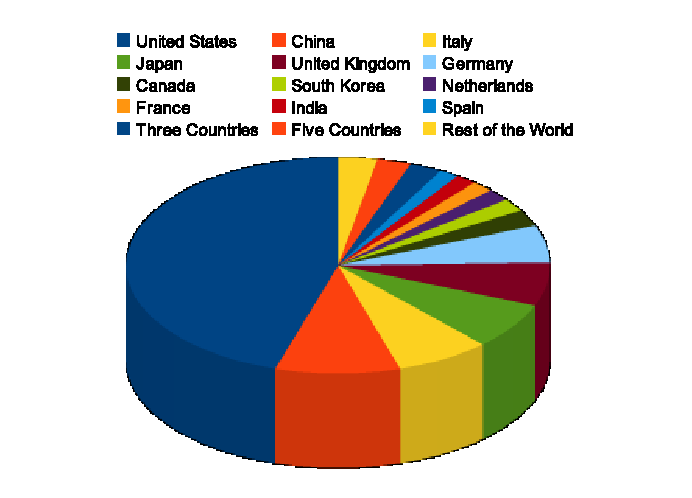
\includegraphics[width=100mm]{part6/Becker_P41/bycountry.eps}
\end{center}
\caption{The 12 top downloading countries, plus three aggregate slices: Three
Countries includes Taiwan, Turkey and Poland; Five Countries comprises Australia,
Mexico, Russian Federation, Greece and South Africa.}
\label{fig:DownloadsByCountry}
\end{figure}

\section{'Bots and Mirrors}

It was obvious from even a cursory glance at the downloads database that Google robots
had been hitting the Chandra archive harder as the mission has progressed - but we wondered
if there were less obvious bulk usages of the archive.

Our ultimate goal was to identify, as much as possible, when downloads were scripted or
automated, as opposed to hand-downloaded. Since mirrors of the Chandra archive (both
official and unofficial / private) have popped up across the globe,\footnote{Italy, India 
and HEASARC currently host official archives; the UK used to have one.} we folded these into the
analysis as well. Some mirrors are not explicitly identified as such, but are easy to spot since
they periodically download the entire archive. Figure~\ref{fig:mirrorsAndBots} is a breakout of activity by year.

\begin{figure}[H]
\begin{center}
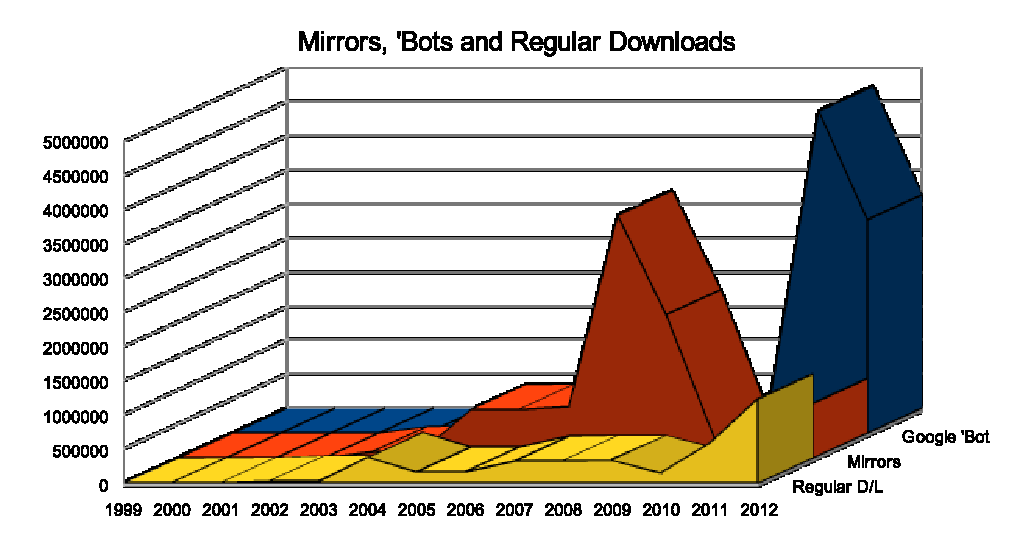
\includegraphics[scale=0.75]{part6/Becker_P41/mirrorbot.eps}
\end{center}
\caption{Web Spider, mirror (official and un-official) and regular download activity compared.}
\label{fig:mirrorsAndBots}
\end{figure}

\section{Conclusion}

We are only beginning to reap the benefits of both tidying up our downloads database
and inserting newly-researched pieces into place. Currently, the database records
each file download as an individual transaction. Going forward we hope to clarify the 
notion of a discrete download session so that we may better understand usage trends. 

The Chandra archive has collected a great deal of data regarding downloads, and our 
modified and strengthened metadata skeleton is giving it much-needed form.

\acknowledgements This work is supported by NASA contract 8-03060.
